\appendix
\section{chktex}
\begin{tiny}
\begin{verbatim}
make[2]: Entering directory '/home/acatejr/workspace/github/cloudmesh-community/hid-sp18-505/project-paper'
cd ../../hid-sample; git pull
Already up-to-date.
cp ../../hid-sample/paper/Makefile .
cp ../../hid-sample/paper/report.tex .
WRNING: line longer than 80 characters
       81:   \centering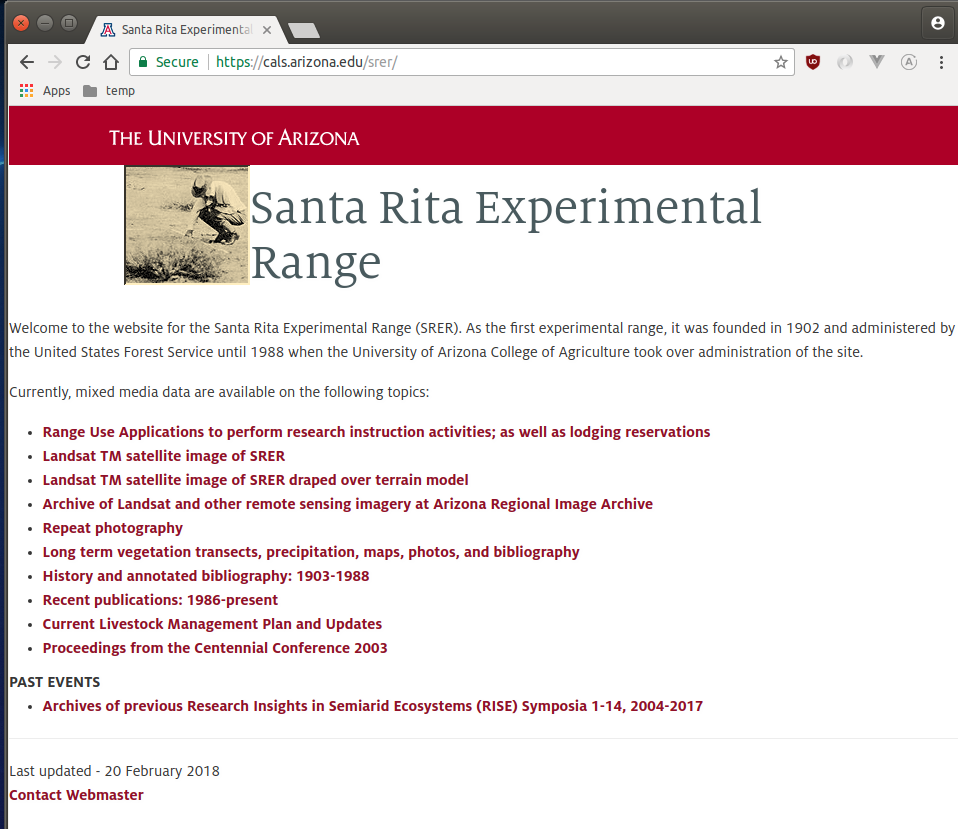
\includegraphics[width=\columnwidth]{./images/srer_landing_page.png}

WRNING: line longer than 80 characters
       85:   \caption{SRER Landing Page\cite{hid505SrerWebSite2018}}\label{f:srer_landing_page}

WRNING: line longer than 80 characters
       85:   \centering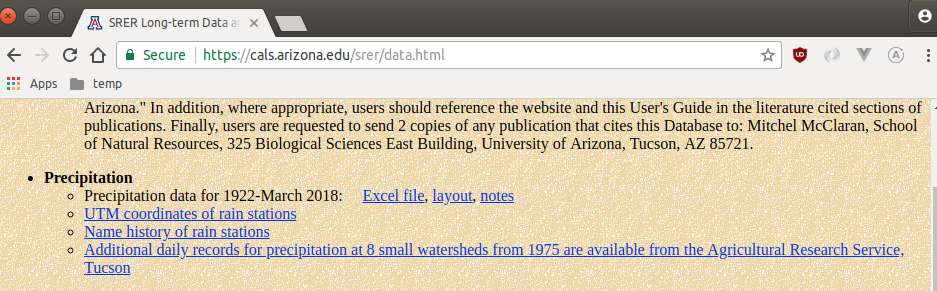
\includegraphics[width=\columnwidth]{./images/srer_precip_data_page.png}

WRNING: line longer than 80 characters
       100:   \caption{SRER Precipitation Data Page\cite{hid505SrerWebSite2018}}\label{f:srer_precip_data_page}

WRNING: line longer than 80 characters
       81: Figure~\ref{f:graphql_rgs} demonstrates an example of a query in the GraphQL UI 

WRNING: line longer than 80 characters
       81: aware of the underlying data model and query request parameters.  Consequently, 

WRNING: line longer than 80 characters
       81: as the user is developing the query, the UI provides autocomplete features that 

WRNING: line longer than 80 characters
       81: delete (CRUD) actions.  GraphQL APIs offer the same type of actions, but not in 

WRNING: line longer than 80 characters
       81: providing support and access to the Walnut Gulch Experimental Watershed website 

make[2]: Leaving directory '/home/acatejr/workspace/github/cloudmesh-community/hid-sp18-505/project-paper'
\end{verbatim}
\end{tiny}
